\documentclass[conference]{IEEEtran}
\IEEEoverridecommandlockouts

\usepackage{amsmath,amssymb,amsfonts}
\usepackage{algorithmic}
\usepackage{graphicx}
\usepackage{textcomp}
\usepackage{xcolor}
\usepackage[style=numeric]{biblatex}

\addbibresource{references.bib}

\begin{document}

\title{Building a Fast Migration System for WireGuard}

\author{
\IEEEauthorblockN{Sina Kamali}
\textit{University of Waterloo}\\
\textit{sinakamali@uwaterloo.ca}
}

\maketitle

\section{Introduction}
WireGuard \parencite[]{Donenfeld2017} is a new tunneling protocol that operates at layer 3 by establishing a Linux virtual network interface. WireGuard provides a fully functioning tunneling system, but it makes an important assumption. WireGuard assumes that peers have a way of exchanging keys. In this work we assume that the broker is in charge of exchanging keys between clients and proxies.

There is not a established way to fast migrate a WireGuard proxy server to another already running proxy server. For a migration system to classify as a fast migration, we require three important factors:

\begin{enumerate}
    \item It should not interfere with other peers that are already connected to the destination proxy.
    \item It should have a low down time for the user.
    \item It should have a low performance cost for the system.
\end{enumerate}

To this end, we designed a novel approach to migrate WireGuard proxies, which will be detailed in full in the following sections.

\section{Design}
To support a fast migration scheme, we create a proxy and client. The proxy connects the client to a NAT server which communicates with the internet on behalf of the client. An overview of this design can be seen in \ref*{fig:odesign}.

\begin{figure}[h]
    \centering
    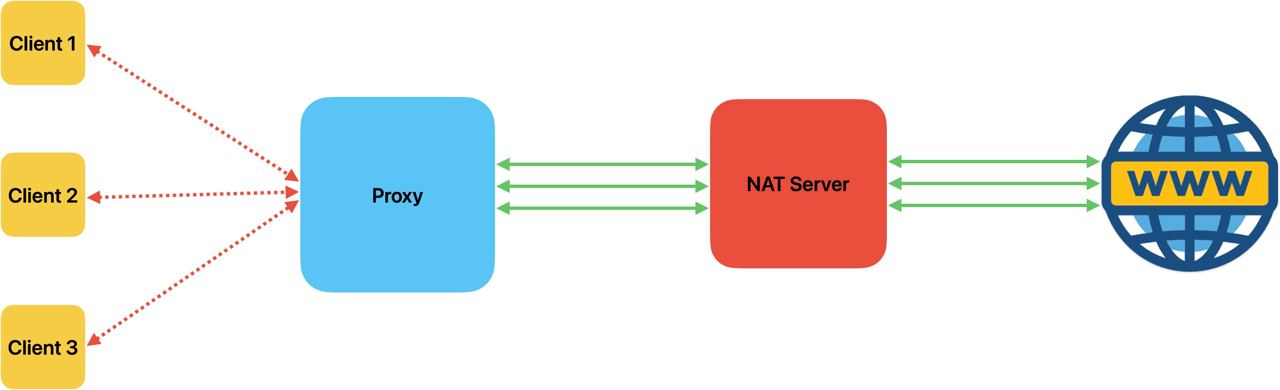
\includegraphics[scale=0.19]{fig1.jpeg}
    \caption{Hierarchical keys}
    \label{fig:odesign}
\end{figure}

\subsection{Designing the Client}
The fast migration client has a few additions on top of a simple WireGuard client. A fast migration client must be able to listen for migration notices from the proxy (to be able to migrate on demand), and should keep track of their last acknowledged sent packet. 

As soon as a WireGuard client receives a migration notice, they disconnect themselves from the old proxy, update their config file, connect to the new proxy, and immediately upon reconnecting, start sending the rest of the packets they were sending that had not been acknowledged. This process happens with minimal down time due to the nature of the WireGuard protocol. The only down time a user encounters in this process is the time it takes for the WireGuard process to restart on their computer, and the time it takes to connect to the new proxy. No other arbitrary slowdowns are present in this protocol.

\subsection{Designing the Proxy}
First off, we have to discuss creating a WireGuard proxy. To do so, we created an application that creates a new thread for each new client. Inside that thread, a two way connection will be established between the client and a NAT server and the proxy will be in charge of sending their messages to each other. This implementation can support any number of clients.

For a WireGuard proxy to support fast migration, not much has to be added except the migration protocol itself. When a proxy decides it is time to migrate a set (or all) of its users to a new proxy the following steps take place:
\begin{itemize}
    \item The proxy sends the clients' WireGuard info from its config file to the destination proxy.
    \item They destination proxy updates its config file.
    \item The first proxy sends a migration request to the set of clients. Inside the migration request, the proxy sends the destination proxy's \textbf{ip} and \textbf{public WireGuard key}.
    \item The first proxy disconnects from the set of clients.
    \item The clients connect to the new proxy as per the steps discussed in the previous section.
\end{itemize}

Following these steps we are able to create a fast migrating WireGuard proxy.


\printbibliography

\end{document}
